\documentclass{article}
\usepackage{graphicx}
\usepackage{amsmath}
\usepackage{hyperref}
\usepackage{subcaption}

\begin{document}

\title{Manual: Vector Field Analysis}
\author{Kota Miura\\
Centre for Molecular and Cellular Imaging\\
EMBL Heidelberg\\
 \texttt{miura@embl.de}\\
Tel. +49 6221 387 404
}

\maketitle

%\label{manual-vector-field-analysis}

Document Date: 2010-10-04

\tableofcontents

\section{Features}\label{features}

\begin{itemize}
\item
  IgorPro (Wavemetrics)\footnote{\url{http://www.wavemetrics.com}}
  Procedure.
\item
  Optical Estimation by temporal local optimization.
\item
  Plotting of vectors in the original video frame.
\item
  Filtering of the vectors by image intensity, velocity and direction.
\item
  Image masking.
\item
  Histograms of velocity, directionality.
\item
  Calculation of protein flow rates.
\end{itemize}

\begin{center}\rule{0.5\linewidth}{\linethickness}\end{center}

\section{Introduction}\label{introduction}

The vector field analysis program uses an algorithm that is called the
optical flow estimation (Teklap, 1995). Optical flow is ``the
distribution of apparent velocities of movement of brightness patterns
in an image'' (Horn and Schunck, 1981). In video sequences the
projection of temporal axis to the \emph{x-y} plane results in an
optical flow image. Since the optical flow is a result of the movement,
it contains information on movement speed and direction. The optical
flow estimation recovers these quantitative measures of the movement,
which enables the statistical treatments of all movement that occurs in
the sequence. A velocity vector field is the calculation result in which
every movement, namely speed and direction, within the sequence is
mapped. The largest difference to the other tracking technique is that
this operation does not require the segmentation step.

Optical flow detection can be categorized into two types in terms of
basic algorithm: the \textbf{matching method} and the \textbf{gradient
method}. In the \textbf{matching method}, displacement is measured by
searching for a particular region in the consecutive frame by matching
the pattern of the previous frame. In the \textbf{gradient method},
optical flow is detected by assuming no changes in the signal intensity
pattern at different time points and by using equations that correlate
the spatial and temporal intensity gradient. This program uses the
gradient method. Details are described elsewhere (Miura, 2005).

Briefly, a general assumption in the gradient method is that the total
intensity of the image sequence is constant.

\begin{equation}
\frac{\partial I(x, y, t)}{\partial x}u + \frac{\partial I(x, y, t)}{\partial y}v + \frac{\partial I(x, y, t)}{\partial t} = 0
\end{equation}
\begin{equation}
\mathbf{v}(u,v)= \mathbf{v}(\frac{dx}{dt},\frac{dy}{dt})
\end{equation}



Where \(I(x,y,t)\) is the intensity distribution of the image and
\(\mathbf{v}\) is the optical flow vector. The equation (1) links the
partial derivatives of the brightness pattern of the image sequence and
the optical flow velocity. Since there are two unknowns, another
constraint is required.

The temporal local optimization method (TLO) used in this program
assumes that the optical flow field is constant temporally (Fig.6)
(Nomura et al., 1991).

\begin{equation}
  \frac{\partial \mathbf{v}}{\partial t} = 0
\end{equation}

The constant vector can be assumed for \emph{N} frames. Then for a stack
with frames , following error function can be generated:

\begin{equation}
  E = \sum_k(I_x(i, j, k)u+I_y(i, j, k)v + I_t(i, j, k))^2
\end{equation}

By the least squared method, \(\mathbf{v}(u,v)\) can be determined by
two equations \(\partial E / \partial u = 0\) and
\(\partial E / \partial v = 0\).

A series of tiff-format image frames is converted to a stack, which is
then treated as a three-dimensional matrix \(I(x,y,t)\). Partial
derivatives of the image sequence must be first calculated as seen in
equations 1 and 4. There are three popular ways for obtaining the
first-order partial derivatives\footnote{\href{http://homepages.inf.ed.ac.uk/rbf/HIPR2/sobel.htm}{Sobel
  filter}}; Sobel kernel, Roberts kernel and Prewitt kernel (also is
called two-point central difference kernel). The Prewitt kernel was used
as follows:

\begin{subequations}
\begin{align}
\frac{\partial I}{\partial t} = \bigg{[}\sum^1_{i=-1}\sum^1_{j=-1}\big{\{}I(x+i, y+j, t+1) - I(x+i, y+j, t-1)\big\}/2\bigg{]}/9
\\
\frac{\partial I}{\partial x} = \bigg{[}\sum^1_{j=-1}\sum^1_{k=-1}\big{\{}I(x+1, y+j, t+k) - I(x-1, y+j, t+k)\big\}/2\bigg{]}/9
\\
\frac{\partial I}{\partial y} = \bigg{[}\sum^1_{i=-1}\sum^1_{k=-1}\big{\{}I(x+i, y+1, t+k) - I(x+i, y-1, t+k)\big\}/2\bigg{]}/9
\end{align}
\end{subequations}

\section{workflow}\label{sec:workflow}

\subsubsection{Preprocessing}\label{preprocessing}

For a successful analysis, following preprocessings are recommended:

\begin{enumerate}
\def\labelenumi{\arabic{enumi}.}
\item
  Check average intensity fluctuation of the sequence (recommended: see
  \hyperref[app1]{Appendix 1}).
\item
  Generate ``Image Mask'' using ImageJ (Fig. \ref{fig:imageMask}: see
  \hyperref[app5]{Appendix 5}). You might not need this if there is no
  background area in the image.
%\end{enumerate}

\begin{figure}[!ht]
\begin{center}

\includegraphics[scale=0.4]{img/image023.png}
\caption{ The ``image filter'' should look something like this. White area
  will be calculated for vector field. Such masking is required since
  noise in the background causes tiny vectors that contaminate the
  measurements.}
\label{fig:imageMask}
\end{center}
\end{figure}

%\begin{itemize}
%\itemsep1pt\parskip0pt\parsep0pt
%\item
%  
\includegraphics{img/image023.png}
%\item
%  Fig.1
%\end{itemize}

%\begin{enumerate}
%\def\labelenumi{\arabic{enumi}.}
%\setcounter{enumi}{2}
\item
  Determine the range of frames to use for the Vector Field analysis by
  inspecting different time points of the stack. Check the shutter
  timing as well (\hyperref[app3]{App.3}). A large fluctuation in the
  image intensity, avoid using those time points.
\item
  It is strongly recommended to do the walking-averaging of the sequence
  to decrease the noise (\hyperref[app4]{App. 4}).
\item
  If required, adjust contrast (\hyperref[app2]{App.2}).
\end{enumerate}

\subsubsection{Setting up the Vector Filed Program in IGORPro
(Compiling)}\label{setting-up-the-vector-filed-program-in-igorpro-compiling}

In IgorPro, do \textbf{{[}File \textgreater{} Open File \textgreater{}
Procedure\ldots{}{]}} and select the file ``\textbf{vec9.ipf}''. Then
click ``Compile'' at the left-bottom corner of the opened procedure
window. In the menu bar, ``Vector field'' and ``Directionality''
appears.

\textbf{Tip:} If compiling does not work, it could be that other procedure
files (.ipf files) are not in the reference path. Check ``User
\textgreater{} Procedures'' folder, and see if the folder containing
Vec9.ipf is linked or copied in that folder.

%\begin{itemize}
%\itemsep1pt\parskip0pt\parsep0pt
%\item
%  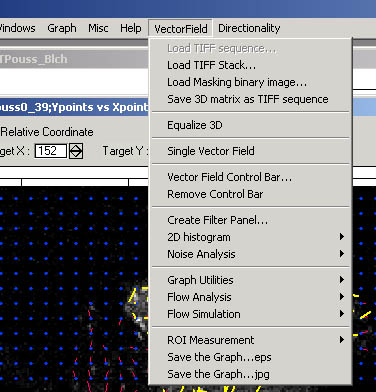
\includegraphics{img/VecFieldMenu.jpg}
%\item
%  Fig. Vector Field analysis menu
%\end{itemize}

\begin{figure}[!ht]
\begin{center}
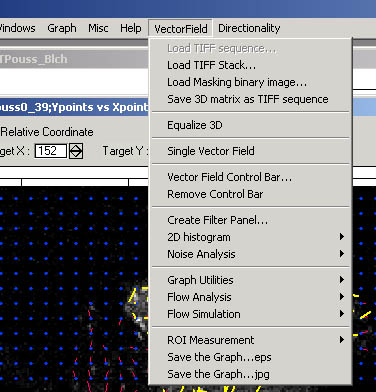
\includegraphics[scale=0.6]{img/VecFieldMenu.jpg}
\caption{ The menu tree of vector field analysis}
\label{fig:vecfieldMenu}
\end{center}
\end{figure}


\subsubsection{Vector Field Analysis}\label{vector-field-analysis}

\begin{enumerate}
\def\labelenumi{\arabic{enumi}.}
\item
  Import a image stack by \textbf{{[}VectorField \textgreater{} Load
  Tiff Stack{]}}.
\item
  Import the image mask in the Vector Filed Analysis Program in the
  IGORPro. \textbf{{[}VectorField \textgreater{} Load Masking binary
  image\ldots{}{]}}
\end{enumerate}

\begin{itemize}
\itemsep1pt\parskip0pt\parsep0pt
\item
  Image Filter can be inverted by {[}VectorField \textgreater{} 2D
  histogram \textgreater{} Invert Mask{]}. This function is sometimes
  convenient since one might prepare a mask which selects only the
  background of the sequence.
\end{itemize}

\begin{enumerate}
\def\labelenumi{\arabic{enumi}.}
\setcounter{enumi}{2}
\itemsep1pt\parskip0pt\parsep0pt
\item
  Calculate the vector field by \textbf{{[}VectorField \textgreater{}
  Single Vector Field{]}}. In a window that pops-up, select the
  tiff-stack, input the frame range (normally, I use 30 frames by
  experience that this is sufficient number of frames). Choose Bleaching
  Correction ``\textbf{linear fit}'', if there is a bleaching of the
  sequence. Other parameters do not have to be changed now.
  ``Averaging'' and ``Scaling'' could be adjusted later after the main
  calculation.
\end{enumerate}

\begin{figure}[!ht]
\begin{center}
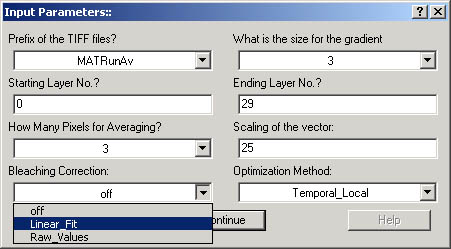
\includegraphics[scale=0.6]{img/veccalcPara041216.jpg}
\caption{ Interface of Vector Field Analysis}
\label{fig:vecfieldGUI}
\end{center}
\end{figure}

\begin{itemize}
\itemsep1pt\parskip0pt\parsep0pt
%\item
%  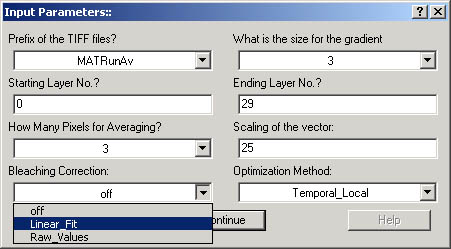
\includegraphics{img/veccalcPara041216.jpg}
\item
  It takes a while to calculate the vector field. While then there will
  be a rotating-disc icon indicating that the calculation is going on,
  at the right bottom corner of the IgorPro window (Fig. \ref{fig:computationDisk}).
%\item
%  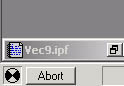
\includegraphics{img/calculationmeter.jpg}

\begin{figure}[!ht]
\begin{center}
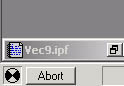
\includegraphics[scale=0.6]{img/calculationmeter.jpg}
\caption{ The icon indicating the process of computation.}
\label{fig:computationDisk}
\end{center}
\end{figure}

\item
  If this calculation is first time in the current igor-experiment, then
  IgorPro asks you for a path to load noise reference data (Fig. \ref{fig:noisedataPathsetter}).
%\item
%  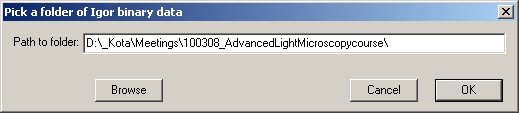
\includegraphics{img/image030.png}

\begin{figure}[!ht]
\begin{center}
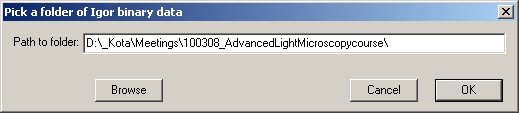
\includegraphics[scale=0.6]{img/image030.png}
\caption{ The interface for setting path to noise data.}
\label{fig:noisedataPathsetter}
\end{center}
\end{figure}

\item
  To set path, click `Browse' button and select ``NoiseParameter''
  folder within Vec9 folder.
\item
  After the calculation, a new Vector Field window appears (fig. \ref{fig:initialVF}).
%\item
%  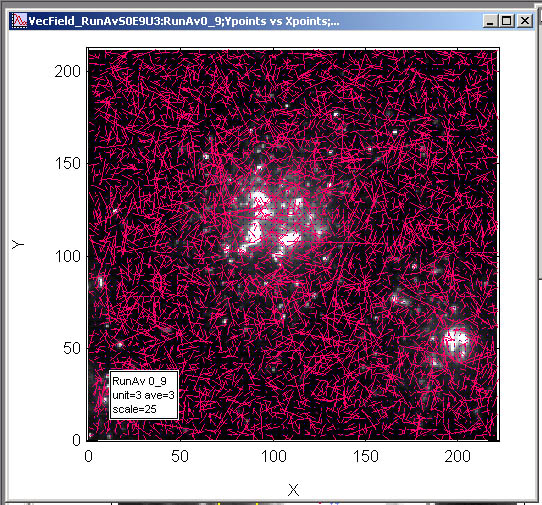
\includegraphics{img/image032.jpg}
\item
  There will be also two new windows, one for the speed histogram and
  another for the direction histogram (fig. \ref{fig:histograms}).
%\item
%  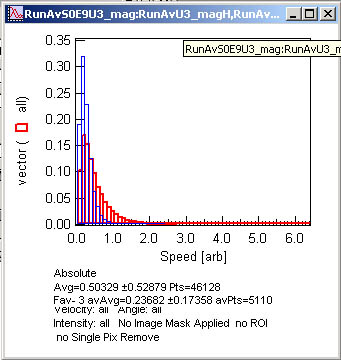
\includegraphics{img/image034.jpg} 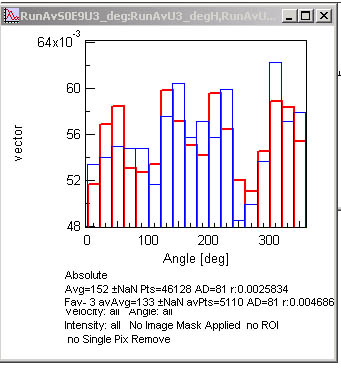
\includegraphics{img/image036.jpg}
\end{itemize}

\begin{figure}[!ht]
\begin{center}
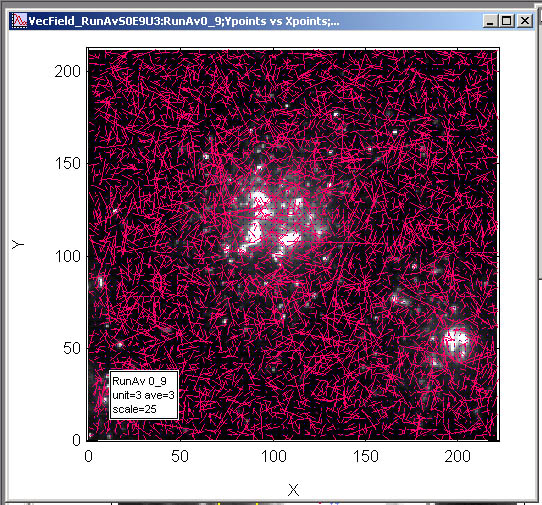
\includegraphics[scale=0.4]{img/image032.jpg}
\caption{ The initial vector field. In general, it needs scaling and filtering for a better view of vectors.}
\label{fig:initialVF}
\end{center}
\end{figure}

\begin{figure}[!ht]
\begin{subfigure}{.5\textwidth}
  \centering
  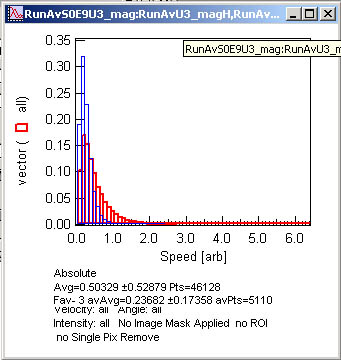
\includegraphics[width=.8\linewidth]{img/image034.jpg}
  \caption{Histogram of speeds.}
  \label{fig:speedHist}
\end{subfigure}%
\begin{subfigure}{.5\textwidth}
  \centering
  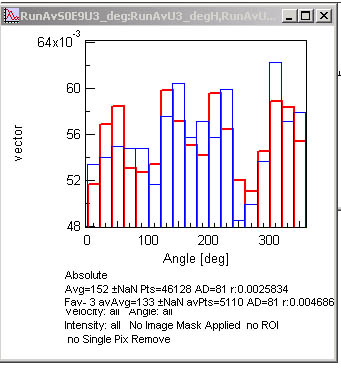
\includegraphics[width=.8\linewidth]{img/image036.jpg}
  \caption{Histogram of angles.}
  \label{fig:angleHist}
\end{subfigure}
\caption{Vector Field analysis results.}
\label{fig:histograms}
\end{figure}

\begin{enumerate}
\def\labelenumi{\arabic{enumi}.}
\setcounter{enumi}{3}
\item
  To decrease the visualized vectors, adjust the vector scaling and
  averaging higher. To do so, activate the vector field window and then
  do \textbf{{[}VectorField \textgreater{}Vector Field Control
  Bar\ldots{}{]}}. This will append a header bar at the top of the
  vector field plot, and averaging and scaling of vectors could be
  adjusted interactively.

\end{enumerate}

\subsubsection{OPTIONAL:  Compute the angle distribution against a reference point.}


 Within the Vector Field Control Bar, select ``Statistics''
  from the pull-down menu. Check ``relative'', then input the
  coordinates for the reference points. The coordinates can be measured
  easily by making a target ROI in the vector field, right click the
  mouse button within that ROI. A menu will appear and choose
  ``V\_show\_ROI\_center'' (fig \ref{fig:setRefPoint}). The centroid coordinates of the selected ROI will be printed in the History window. Input those values in ``TargetX'' and ``TargetY'' (fig. \ref{fig:targetXY}). Clicking ``Do it'' button will change the measurement of direction of the vectors against the reference point.
%\end{enumerate}

%\begin{itemize}
%\item
%  \begin{figure}[htbp]
%  \centering
%  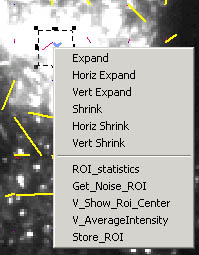
\includegraphics{img/image038.jpg}
%  \caption{}
%  \end{figure}
%\item
%  The centroid coordinates of the selected ROI will be printed in the
%  History window. Input those values in ``TargetX'' and ``TargetY''.
%  Clicking ``Do it'' button will change the measurement of direction of
%  the vectors against the reference point.
%\item
%  \begin{figure}[htbp]
%  \centering
%  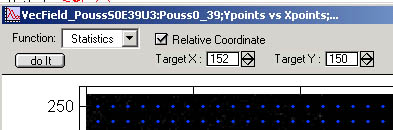
\includegraphics{img/image040.jpg}
%  \caption{}
%  \end{figure}


\begin{figure}[!ht]
\begin{subfigure}{.3\textwidth}
  \centering
  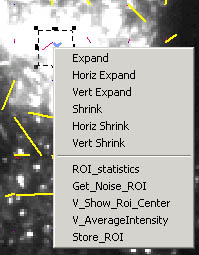
\includegraphics[width=.8\linewidth]{img/image038.jpg}
  \caption{Selecting reference point.}
  \label{fig:setRefPoint}
\end{subfigure}%
\begin{subfigure}{.7\textwidth}
  \centering
  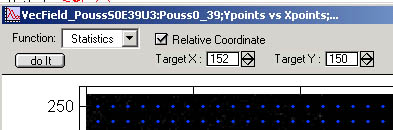
\includegraphics[width=.8\linewidth]{img/image040.jpg}
  \caption{The interface for setting reference coordinates.}
  \label{fig:targetXY}
\end{subfigure}
\caption{Optional: computing vector angles against a reference point.}
\label{fig:referenceSettings}
\end{figure}

The direction histogram changes its range from 0 - 360º to -180º -
+180º. In the latter case, 0º is directed towards the reference point,
and ±180º is directed away from the reference point (fig. \ref{fig:relativeAngleHIst}).


%\item
%  \begin{figure}[htbp]
%  \centering
%  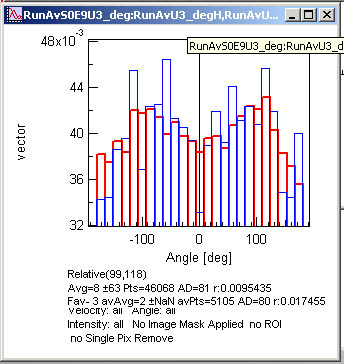
\includegraphics{img/directionhist_relative.jpg}
%  \caption{}
%  \end{figure}
%\end{itemize}

\begin{figure}[!ht]
\begin{center}
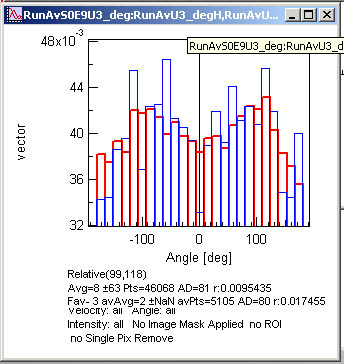
\includegraphics[scale=0.4]{img/directionhist_relative.jpg}
\caption{ Histogram of vector angles measured against a reference point}
\label{fig:relativeAngleHIst}
\end{center}
\end{figure}

%\begin{enumerate}
%\def\labelenumi{\arabic{enumi}.}
%\setcounter{enumi}{5}
%\itemsep1pt\parskip0pt\parsep0pt

\subsubsection{OPTIONAL: Vector Filtering} 

If vector field is influenced by noise largely,
  these noise derived information must be removed from the measurement.
  To do so, do \textbf{{[}VectorField \textgreater{} Create Filter
  Panel\ldots{}{]}}. This then pops up a window titled ``Filter Panel'' (fig. \ref{fig:vecfilterGUI}).
  There are several types of filters and you can set their parameter to
  remove noise derived vectors.
%\end{enumerate}
%
%\begin{itemize}
%\itemsep1pt\parskip0pt\parsep0pt
%\item
%  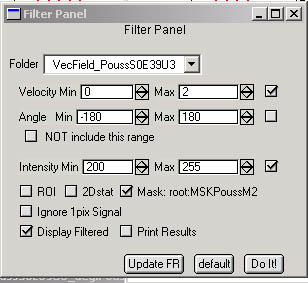
\includegraphics{img/filterpanel.jpg}
%\end{itemize}
%

\begin{figure}[!ht]
\begin{center}
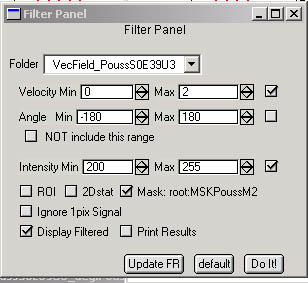
\includegraphics[scale=0.7]{img/filterpanel.jpg}
\caption{ Vector filtering panel.}
\label{fig:vecfilterGUI}
\end{center}
\end{figure}

\begin{enumerate}
%\def\labelenumi{\arabic{enumi}.}
\item
  Find the optimum lower and higher limit for the intensity filter
  (compare the original movie and the vector field). Input the values
  within the Filter Panel. For selecting intensity range, threshold
  function in ImageJ is useful \textbf{{[}Image \textgreater{} adjust
  \textgreater{} threshold{]}}.
\item
  Find the ``speed of noise'' from the back ground and set the lower
  limit for the speed detection. Input the value in the Filter Panel.
\item
  Set the image-filter by checking the ``Mask'' check box. A dialogue
  window will appear. Select the Image Mask from the pull down menu.
\item
  Don't forget to check the ``Display Filtered'' check box.
\item
  Click ``Do it'' to execute the filtering. After the filtering is done,
  yellow vectors will appear, which are the vectors after the filtering.
  Statistics will also change, showing only the results from those
  yellow vectors.
\item
  Filtering parameters can be changed and re-calculated.
\end{enumerate}

\subsubsection{OPTIONAL: Flow Rate calculation}
\begin{enumerate}
\item
  Check the background intensity. Move the curser to the background
  region of the vector field, click right mouse button and select
  ``V\_AverageIntensity'' form the menu. The average background
  intensity will appear in the command window.
\item
  Set background intensity by VectorField Flow Analysis Set Background
  Intensity.
\item
  Do the analysis by VectorField Flow Analysis Calculate Flow. New
  graphs will appear.
\end{enumerate}

\section{Appendix}
\label{appendix}

\label{subsec:app1}
\subsection{Appendix 1: Checking the average intensity fluctuation.}

\textbf{Dealing with Image Sequences with Blinking (Fluctuation of the
fl. Intensity)}

One could measure the temporal changes in the average intensity of
frames in the following way using ImageJ. First, open the stack that you want to measure. Then a macro program should be installed.

\textbf{{[}Plugins Macros Install\ldots{}{]}}

Then a popup window appears and a file called
``\textbf{StackManager.txt}'' must be chosen from wherever it is saved.
This file could be downloaded from

\url{http://cmci.embl.de/dls/StackManager.ijm}

as well (right click and ``save link as'').

You will see new commands in the Macros menu {[}Plugins \textgreater{}
Macros \textgreater{} \ldots{}{]} (fig. \ref{fig:ijmenuMacro}).

\begin{figure}[!ht]
\centering
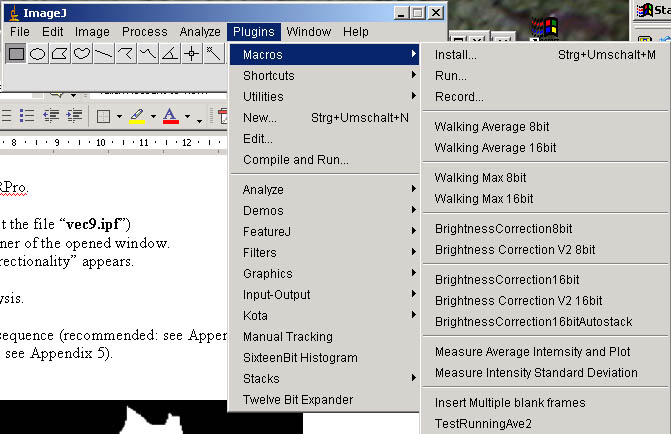
\includegraphics[scale=0.3]{img/image046.jpg}
\caption{Installed macro appears in the ImageJ menu.}
\label{fig:ijmenuMacro}
\end{figure}

Activate the Stack window by clicking the title bar, and then select
``\textbf{Measure Average Intensity and Plot}'' form the macro menu. The
program goes through the sequence once and then there will be a new
window (fig. \ref{fig:intensityTimeCourse}).

%\begin{figure}[htbp]
%\centering
%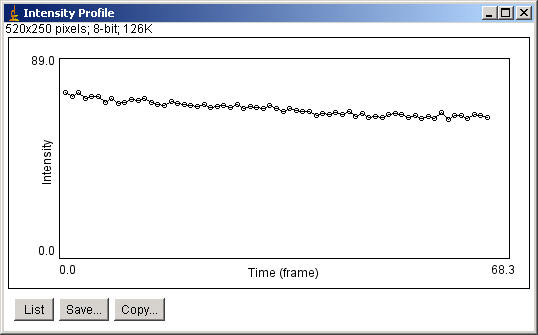
\includegraphics{img/image048.png}
%\caption{}
%\end{figure}

\begin{figure}[!ht]
\centering
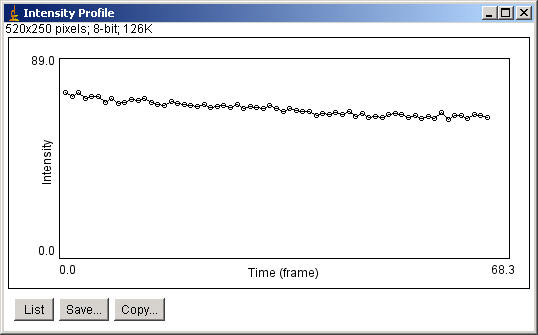
\includegraphics[scale=0.3]{img/image048.png}
\caption{Intensity changes over time.}
\label{fig:intensityTimeCourse}
\end{figure}


This plot shows how the average intensity of your sequence changes from
frame to frame. The average intensity is decreasing, because there is a
slight acquisition-photobleaching of the fluorescence.

In some cases, the intensity fluctuates largely. This could be caused by
several reasons such as unstable light source (this happens a lot with
old lamps) or changes in the focus plane. In any case, avoid using such
a sequence, or use only a part of the sequence with a constant intensity
(or with a constant photo-bleaching rate)

\subsection{Appendix 2: Enhancing contrast and down-scaling from 16 bit to 8bit}

This section explains how to convert 16-bit image sequences to 8-bit for faster computation of vector field. Note that this processing changes pixel intensity, so if you need to treat pixel intensity for measurement of protein density (such as for flow rate estimation), avoid this processing. 

\begin{enumerate}

\item Open 16bit Tiff Sequence as a Stack in ImageJ.

\item Select a frame at a position about 2/3\textsuperscript{rd} of the whole
sequence.

\item Check that the selected frame is not extraordinarily bright or dark compared to other frames.

\textbf{{[}Analyze \textgreater{} Histogram{]}}

This command displays an intensity histogram of the image. In most of images from fluorescence microscopy, histogram has a narrow peak towards left-side with a long tail towards the right side of the histogram. 

Since this is a 16bit image, Grayscale has 65536
(=2\textsuperscript{16}) steps between black(0) and white(65535) You
need to down scale this and set a full rage in 8 bit, which consists of
256 (=2\textsuperscript{8}) steps.

For example, if histogram of a frame distributes in a range of pixel
values between 82 and 1009 (``min'' and ``max''), it means that there are ca. 900 gray scale in the image. Such a wide scale might not be necessary for your analysis as the range of the target signal might be narrower. To determine this meaningful range, the histogram must be examined carefully. You could use two different ways.

\begin{itemize}
\item \textbf{Interactive pixel value reading}: Hover the mouse cursor
over the histogram. As you move your cursor across the histogram, you will notice that ``Value'' (= pixel value) indicated below the histogram changes dynamically e.g.~if your cursor is at ``Value'' 328 and ``Count'' is 26, it means that the number of pixels with a pixel value 328 in the image is 26 pixels. As you move your cursor closer to the peak, ``Count''
starts to increase. e.g.~the ``Value'' is 165, ``Count'' is 435, and so
on. Compare the value readout and actual pixels values in the image to
figure out the pixel value range that you are interested in.

In an example case fig. \ref{fig:checkPixelValues}, the right side was determined to be ``Value''=144 and the left side at ``Value''=86.

%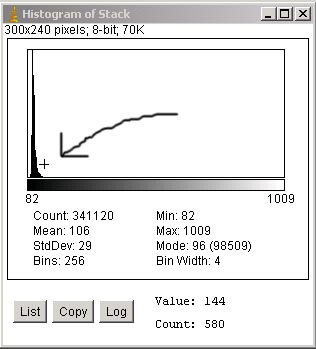
\includegraphics{img/image050.jpg} Fig. A2-1

\begin{figure}[!ht]
\centering
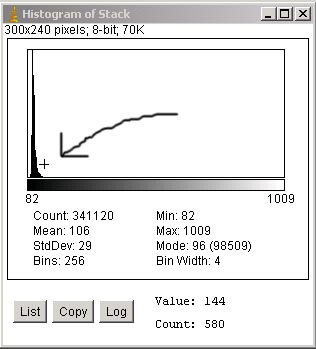
\includegraphics[scale=0.4]{img/image050.jpg}
\caption{Checking pixel values using histogram window.}
\label{fig:checkPixelValues}
\end{figure}


\item \textbf{Numerical readout}: Click the ``List'' button in the histogram
window. A list of number appears. This is the actual values of the
histogram. The first column is the ``Value'' and the second column is
the corresponding ``Count'' By examining the histogram values, the
approximate steps that contain the peak position can be determined.
\end{itemize}


\item \textbf{[Image \textgreater{} Adjust \textgreater{}Brightness/Contrast]}

This command displays Brightness and Contrast adjustment GUI. Click
``Set'' button. A small window pops-up. Set the ``Minimum Displayed
Value'' to 86 and the ``maximum displayed value'' to 144. Now you see
that the Image is contrast enhanced. Note that this only changes the LUT, not the pixel values of the image. 

\item To apply this LUT and convert the image to 8-bit, choose the following command. 

\textbf{{[}Image \textgreater{} Type \textgreater{} 8bit{]}}

\item Check that pixel values are changed. 

\textbf{{[}Analyze \textgreater{} Histogram{]}}

The histogram should be nicely distributed between the value 0
and 255.
\end{enumerate}

%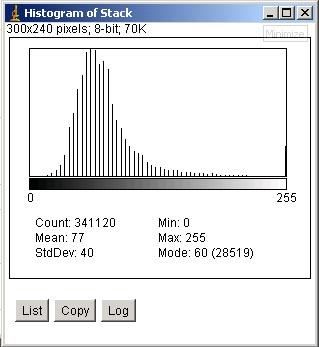
\includegraphics{img/image052.jpg} Fig. A2-2
\begin{figure}[!ht]
\centering
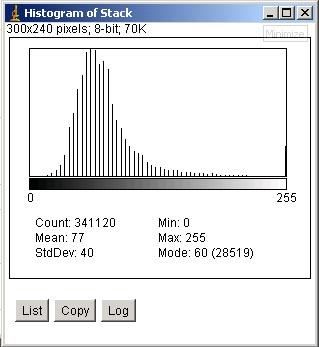
\includegraphics[scale=0.4]{img/image052.jpg}
\caption{The histogram after conversion to 8-bit.}
\label{fig:postconversion}
\end{figure}


\subsection{Appendix 3: Checking the shutter timings.}

Some sequences contain ``blinking'' of the frames. This could be due to

\begin{enumerate}
\def\labelenumi{\arabic{enumi}.}
\itemsep1pt\parskip0pt\parsep0pt
\item
  Light-source shutter is unstable.
\item
  Camera shutter is unstable.
\item
  Light source itself is blinking.
\item
  Focusing position changed.
\end{enumerate}

To evaluate the stability of camera shutter timings, one can go back to the shutter log (``time stamps'') and check if the sequence was taken with a constant shutter timings (fig. \ref{fig:dtplot}).

%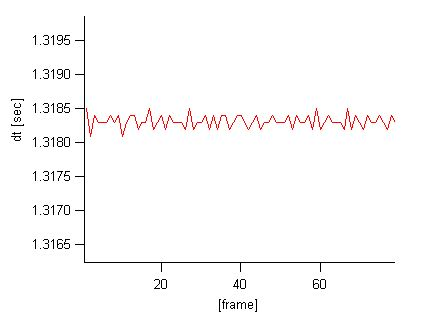
\includegraphics{img/image054.jpg} Fig. 

\begin{figure}[!ht]
\centering
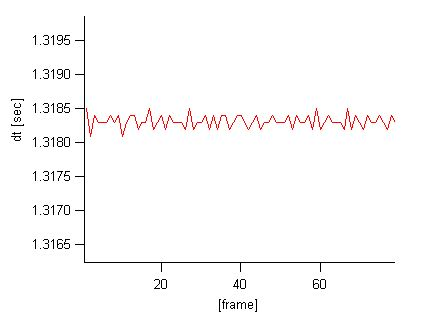
\includegraphics[scale=0.4]{img/image054.jpg}
\caption{$dt$ plot generated from the``.tim'' file.}
\label{fig:dtplot}
\end{figure}


\subsection{Appendix 4: Walking average.}

Walking averaging of a image sequence converts each frame of the
sequence to an average of successive frames.

This file could be downloaded from

\url{http://cmci.embl.de/dls/StackManager.ijm}

After installing the macro, ImageJ macro menu looks like figure \ref{fig:stackmanagerMenu}.

\begin{figure}[!ht]
\centering
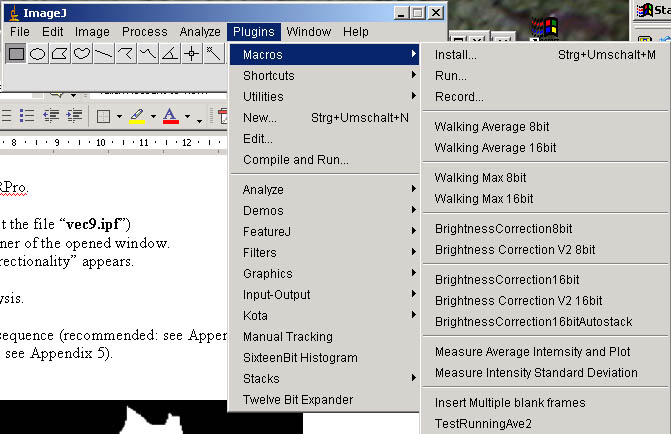
\includegraphics[scale=0.4]{img/StackmanagerMenu.jpg}
\caption{Stackmanager in ImageJ menu.}
\label{fig:stackmanagerMenu}
\end{figure}


If the bit-depth of your image stack is 8-bit, choose ``Walking average 8 bit'' If 16bit, choose ``Walking average 16 bit''. Then a pop-up window appears (fig \ref{fig:waparameters})

\begin{figure}[!ht]
\centering
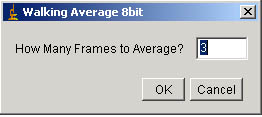
\includegraphics[scale=0.6]{img/Stackmanager_waPOP.jpg}
\caption{Stackmanager in ImageJ menu.}
\label{fig:waparameters}
\end{figure}

Input number of frames that you want to average, then click ``OK''. A
new stack appears that is walking averaged.

\subsection{Appendix 5: Generating a Image Mask for Vector field.}

To make image mask, you need to use ImageJ. First, you must make two
copies of a frame in the sequence you want to analyze. This can be done
by

\textbf{{[}Image \textgreater{} Duplicate\ldots{}{]}}

This will create a copy of the frame in the stack. If image is not
8-bit, then convert the image to 8 bit by

\textbf{{[}Image \textgreater{} Type \textgreater{} 8bit{]}}

Using this duplicated frame, you need to trace the edge of the cell.
This is done by selecting freehand tool. Click the freehand ROI icon in
the ImageJ menu bar (fig. \ref{fig:freehandROIicon}).

\begin{figure}[!ht]
\centering
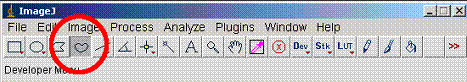
\includegraphics[scale=0.5]{img/image060.jpg}
\caption{Selecting freehand ROI tool.}
\label{fig:freehandROIicon}
\end{figure}

Then trace the cell edge like figure \ref{fig:celledgeTraced}.

%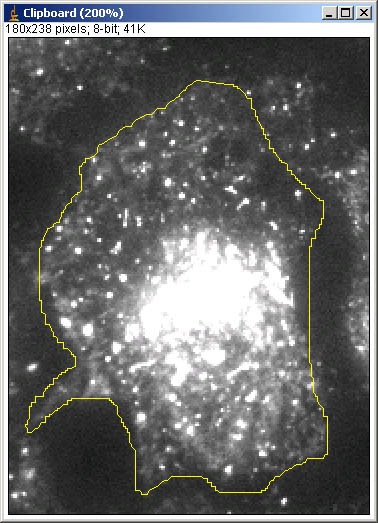
\includegraphics{img/celledgetrace.jpg}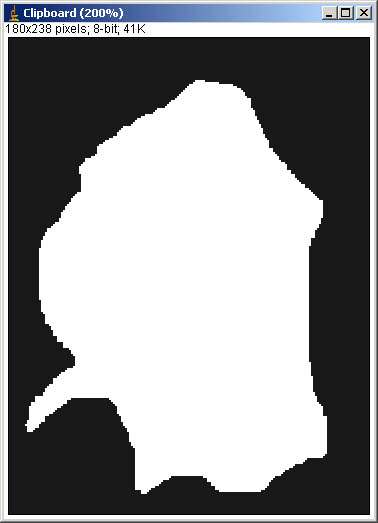
\includegraphics{img/celledgetrace_bw.jpg}

\begin{figure}[!ht]
\begin{subfigure}{.5\textwidth}
  \centering
  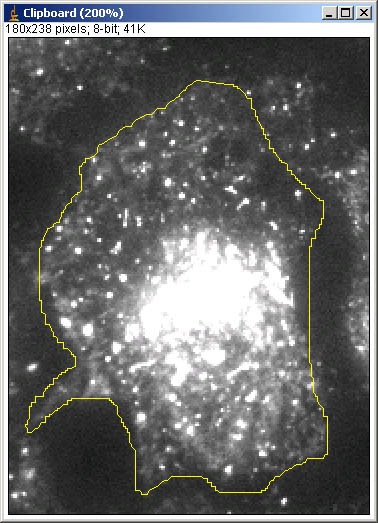
\includegraphics[width=.8\linewidth]{img/celledgetrace.jpg}
  \caption{Cell edge traced using freehand ROI.}
  \label{fig:celledgeTraced}
\end{subfigure}%
\begin{subfigure}{.5\textwidth}
  \centering
  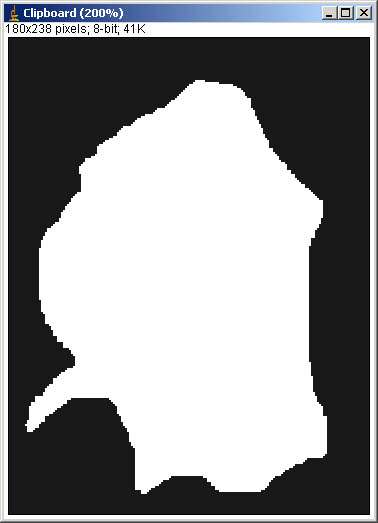
\includegraphics[width=.8\linewidth]{img/celledgetrace_bw.jpg}
  \caption{Generated mask from the trace.}
  \label{fig:celledgeMask}
\end{subfigure}
\caption{Preparing cell mask.}
\label{fig:celledgemaskCreation}
\end{figure}


Then after tracing, do

\textbf{{[}Edit \textgreater{} Fill{]}}

Tip: If inside area of the ROI do not become white, then check color
option by {[}Edit \textgreater{} Options \textgreater{}
Color\ldots{}{]}. Check that the color assignment shown in the window
appeared is like the one shown in figure \ref{fig:colorsettings}.

\begin{figure}[!ht]
\centering
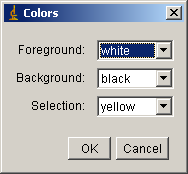
\includegraphics[scale=0.7]{img/image065.png}
\caption{Color settings}
\label{fig:colorsettings}
\end{figure}

Then

\textbf{{[}Edit \textgreater{} Clear outside{]}}

This will fill black in the outside area of selected ROI. By these last
two steps, image should have become black and white (fig. ref{fig:celledgeMask}).

OPTIONAL: masking area inside cell.

Sometimes signal is too high inside cell and this interferes with
yourvector analysis. In such a case, another mask could be prepared to
mask that high-intensity area, and combine it with the cell edge mask
prepared above. You first make another duplicate of a frame by
\textbf{{[}image \textgreater{} duplicate{]}}. Then Trace the high
intensity area, and convert them to black ad white just like the first
one.

%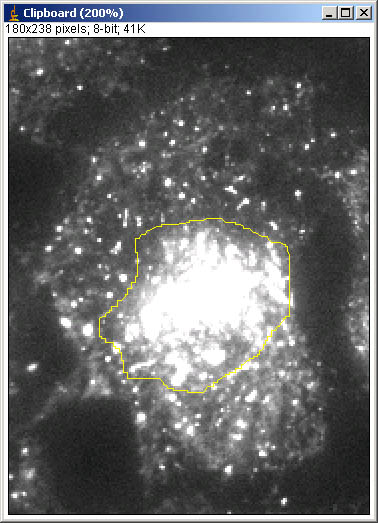
\includegraphics{img/cellnuctrace.jpg}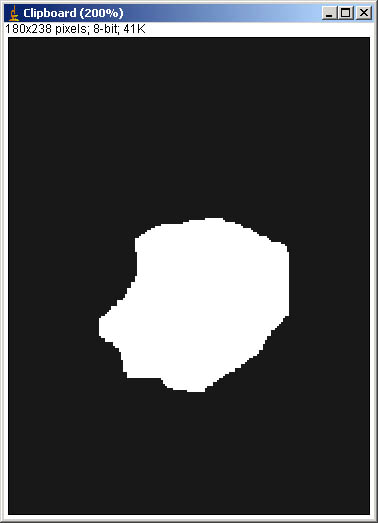
\includegraphics{img/cellnuctrace_bw.jpg}

\begin{figure}[!ht]
\begin{subfigure}{.5\textwidth}
  \centering
  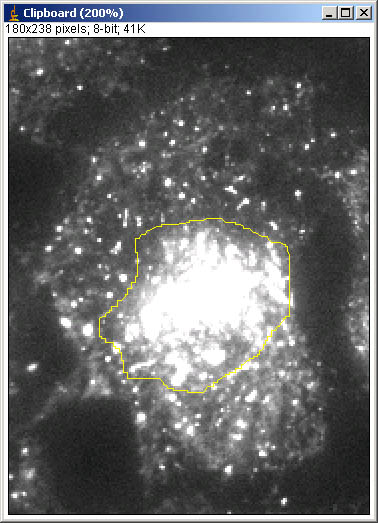
\includegraphics[width=.8\linewidth]{img/cellnuctrace.jpg}
  \caption{Cell nucleus traced using freehand ROI.}
  \label{fig:nucTraced}
\end{subfigure}%
\begin{subfigure}{.5\textwidth}
  \centering
  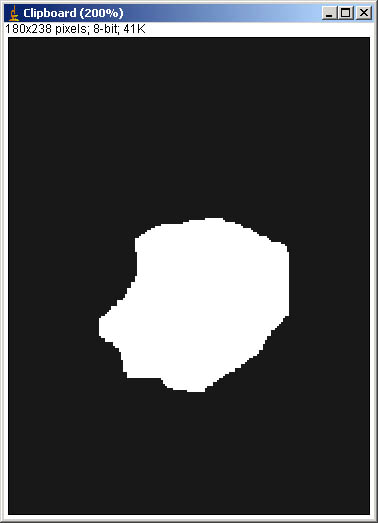
\includegraphics[width=.8\linewidth]{img/cellnuctrace_bw.jpg}
  \caption{Generated nucleus mask from the trace.}
  \label{fig:nucMask}
\end{subfigure}
\caption{Preparing nucleus mask.}
\label{fig:nucmaskCreation}
\end{figure}


Since we do not want to measure the white area, we invert the image so
that the selected area becomes black (fig. \ref{fig:invmask}).

\textbf{{[}Edit \textgreater{} Invert{]}}

\begin{figure}[htbp]
\centering
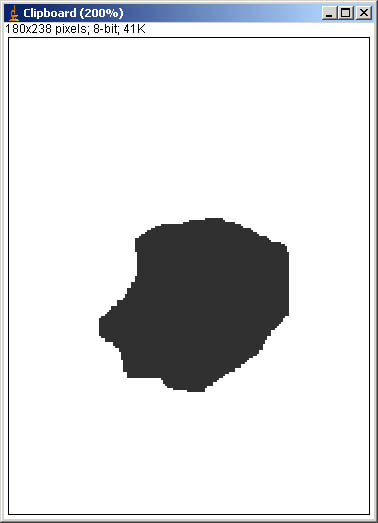
\includegraphics[scale=0.5]{img/cellnuctrace_bw_inv.jpg}
\caption{Inverted mask}
\label{fig:invmask}
\end{figure}

Finally, use Image calculator to combine two masks (fig. \ref{fig:imgcalcGUI}).

\textbf{{[}Process \textgreater{} Image Calculator\ldots{}{]}}

\begin{figure}[htbp]
\centering
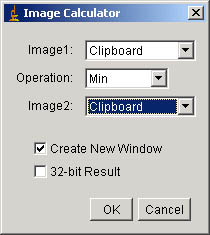
\includegraphics[scale=0.7]{img/imageCalculator.jpg}
\caption{Image Calculator.}
\label{fig:imgcalcGUI}
\end{figure}

Select the first clipboard as image 1 and the second clipboard as the
image 2. Operation is ``Min''. Then the combined image mask is created (fig \ref{fig:finalmask}) and can be
imported from IgorPro.

\begin{figure}[htbp]
\centering
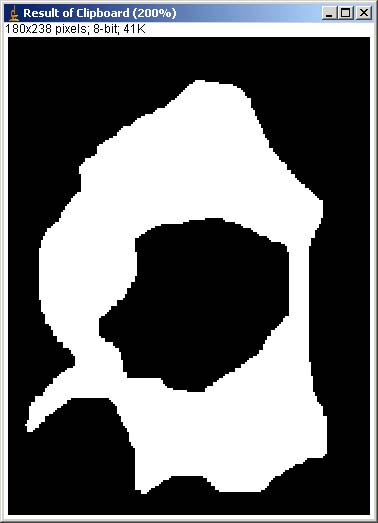
\includegraphics[scale=0.4]{img/maskfinal.jpg}
\caption{Combined mask.}
\label{fig:finalmask}
\end{figure}

\section{References}\label{references}

\textbf{Horn, B. K. P. and Schunck, B. G.} (1981). Determining Optical
Flow. \emph{Artificial Intelligence} \textbf{17}, 185-203.

\textbf{Miura, K.} (2005). Tracking Movement in Cell Biology. In
\emph{Advances in Biochemical Engineering/Biotechnology}, vol.~95 (ed.
J. Rietdorf), pp.~267. Heidelberg: Springer Verlag.

\textbf{Nomura, A., Miike, H. and Koga, K.} (1991). Field theory
approach for determining optical flow. \emph{Pattern Recog. Lett.}
\textbf{12}, 183-190.

\textbf{Teklap, M.} (1995). Digital Video Processing. Englewood Cliffs,
N.J.: Prentice Hall.

\end{document}
